\chapter{Methoden}
\label{methoden}
TODO Methoden GIT, CICD und so erklären und wieso diese hier erwähnt sind:

Für dieses Projekt wurde zu Beginn ein agiles Vorgehen gewählt.
Der Grund dafür war, dass das genaue Projektziel noch nicht klar definiert werden konnte.
Als erstes sollte eine minimaler Prototyp erarbeitet werden. In der Aufgabenstellung (Anhang \ref{anhang:aufgabenstellung}) wurden dafür folgende Aufforderungen definiert:
\begin{itemize}
\item Visualisierung des Spannungsverlaufs (drei Phasen) eines Stromzählers
basierend auf gespeicherten Messdaten.
\item Empfangen (TLS Verschlüsselung) und abspeichern von Messdaten (Spannung über drei Phasen) und
Zeitstempel mittels MQTT.
\item Bereitstellen von virtuellen Stromzählern, welche mittels MQTT Messdaten
übermitteln.
\end{itemize}
Nach ca. einem Drittel der Projektzeit wurde das erarbeitete dem Auftraggeber vorgeführt und die implementierten Funktionalitäten demonstriert.
Gemeinsam mit dem Auftraggeber wurden danach die Anforderungen für die nächste Iteration definiert.
Diese Prinzip wurde noch ein weiteres mal durchgeführt.
Gegen Ende der Projektzeit wurde das Endresultat vom Projektteam präsentiert und eine letzte Rückmeldung von Auftraggeber eingeholt.

% Aus Aufbau_Bericht.pdf
% Hier halten Sie fest und begründen, welches Vorgehensmodell Sie für Ihr Projekt wählen. Sie
% verweisen allenfalls auf die daraus entstandenen, konkreten Terminpläne mit Meilensteinen, welche
% z.B. unter Realisierung (Kapitel 5) oder im Anhang versorgt sind.

% Bei Engineering-Projekten halten Sie weitere einzusetzende fachliche Methoden oder Techniken fest.
% Bei einem Softwareprojekt können dies z.B. der geplante Einsatz einer Anforderungsanalyse, der
% Einsatz von Review-Techniken (Architektur-Reviews) oder bekannter Programmiertechniken sein.


\section{Teststrategie}
\label{teststrategie}

Um sicherzustellen, dass das Projekt jederzeit funktioniert und keine Änderungen
aus Versehen andere Funktionalität beeinträchtigt, werden Automatisierte
End to End Tests erstellt. Bei End to End Tests werden die Tests möglichst
so ausgeführt wie die Applikation auch deployt wird. \parencite{georgian_2021}
Auf andere Tests wie Unit Tests wird in diese Projekt aus zeitgründen verzichtet. TODO

Diese Tests wurden Behaviour Driven implementiert.\footnote{
    Behavior-driven development (BDD) is an Agile software development methodology
    in which an application is documented and designed around the behavior a user
    expects to experience when interacting with it.
} \parencite{what_is_bdd} Die Tests wurden anhand der Anforderungen \ref{aufgabenstellung}
und User Stories in der Gherking Sprache\footnote{https://cucumber.io/docs/gherkin/reference/} implementiert.

\section{Versionskontrolle}

Wie im Softwareengineering Bereich üblich, wurde auch in diesem Projekt mit Git\footnote{https://git-scm.com/}
gearbeitet. Dies ist mittlerweile der de facto Standard um Software Projekte zu versionieren. \parencite{git}
Da das Projekt nur zu zweit realisiert wurde und von keinem grossen Projektteam, wurde auf
eine komplizierte Branching Strategie wie beispielsweise
GitFlow\footnote{https://www.atlassian.com/git/tutorials/comparing-workflows/gitflow-workflow} verzichtet.
Für die Erstellung grösserer Features wurden Branches erstellt und falls nur kleinere
Änderungen gemacht wurden, wurden diese direkt auf den Hauptbranch gepusht.

Diese Arbeit wurde in \LaTeX geschrieben, weswegen sie ebenfalls Versionskontrolliert abgelegt wurde.
Beide Projekte sind Open Source auf GitHub\footnote{https://github.com} abgelegt unt under
folgenden Links zu finden:

\begin{itemize}
  \item Das Projekt: \url{https://github.com/randombenj/hslu-wipro-smic}
  \item Diese Arbeit: \url{https://github.com/randombenj/hslu-wipro-smic-doc}
\end{itemize}

Ob das Projekt direkt Open Source implementiert werden darf, wurde zuvor so mit der Landis+Gyr abgesprochen.

\section{Code Reviews}

Um eine hohe Qualität der Software sicherzustellen, wurde nebst der Teststrategie \ref{teststrategie}
auch Code Reviews und Pair Programming durchgeführt. \parencite{fu2017code}
Die Reviews und Pair Programming sessions wurden jeweils an den wöchentlichen
Meetings (TODO describe) durchgeführt.
Bei den grösseren Fetures bei denen ein eigener Branch erstellt wurde, wurden die
Reviews direkt über einen Pull Request auf GitHub gemacht. \parencite{github_flow_docs_2021}

\subsection{\ac{CI/CD}}

Um das Projekt automatisch Testen zu können und eine Reproduzierbare Umgebung zu bauen,
wurde bereits zu Beginn eine \ac{CI/CD} Pipeline mit GitHub Actions\footnote{https://github.com/features/actions}
aufgebaut.
Die Entwickler sollen sich nicht nur um die Entwicklung, sondern auch das automatische Bauen und Deployen der
Software kümmern. Dieser DevOps Gedanke hat den Vorteil, dass
theoretisch jedes kleine Feature und jeder Bugfix direkt automatisiert getestet
wird und danach (wenn die Tests erfolgreich waren) auf das Produktivsystem
Deployt werden kann. \cite{what_is_devops}
zudem ist für jeden Entwickler das Bauen und Ausführen des Projektes gleich und
reproduzierbar. Dies erspart das Suchen von unnötigen Fehlern die auf unterschiedlich
konfigurierten Entwicklungsmaschinen auftreten können.

TODO konkrete CI pliplie in Iteration1 erklären

\begin{figure}[h]
    \centering
    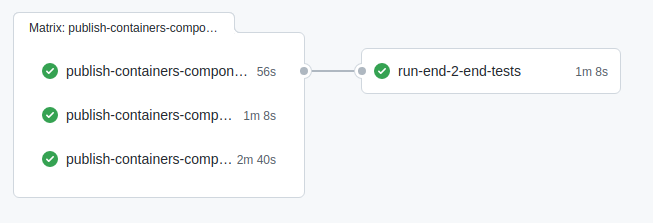
\includegraphics[width=1.0\textwidth]{gfx/ci-env}
    \caption{
        Visualisierung der GitHub Actions Pipeline mit zwei aufeinanderfolgenden Stages.
        Zuerst werden die einzelnen Komponenten (Siehe \ref{fig:smic-arch}) gebaut und
        anschliessend getestet.
    }
    \label{fig:ci-env}
\end{figure}

Dank dieser \ac{CI/CD} Umgebung und der Verwendung von Podman, kann die gesamte Applikation
(Wie im Kapitel \ref{architekturentscheidung} beschrieben) mit einem
Befehl gebaut und gestartet werden.